\documentclass{article}
\usepackage{include/nips15submit_e,times}
\usepackage{hyperref}
\usepackage{url}
\usepackage[noend]{algpseudocode}
\renewcommand\algorithmicthen{}
\renewcommand\algorithmicdo{}
\usepackage{algorithm}
\usepackage{natbib}
\usepackage{graphicx}

\definecolor{mydarkblue}{rgb}{0,0.08,0.45}
\hypersetup{
    colorlinks=true,
    linkcolor=mydarkblue,
    citecolor=mydarkblue,
    filecolor=mydarkblue,
    urlcolor=mydarkblue}

\newcommand{\vw}{\mathbf{w}}
\newcommand{\vv}{\mathbf{v}}
\newcommand{\vf}{\mathbf{f}}
\newcommand{\vg}{\mathbf{g}}
\newcommand{\vi}{\mathbf{i}}
\newcommand{\vr}{\mathbf{r}}
\newcommand{\vzero}{\mathbf{0}}
\newcommand{\ones}[1]{\mat{1}_{#1}}
\newcommand{\eye}[1]{\mat{E}_{#1}}
\newcommand{\tra}{^{\mathsf{T}}}
\newcommand{\vect}[1]{{\bf{#1}}}
\newcommand{\mat}[1]{\mathbf{#1}}
\newcommand{\pderiv}[2]{\frac{\partial #1}{\partial #2}}
\newcommand{\npderiv}[2]{\nicefrac{\partial #1}{\partial #2}}

\title{Neural Molecular Fingerprints}

\author{
David Duvenaud\\
Harvard University\\
\texttt{dduvenaud@seas.harvard.edu}
\And
Dougal Maclaurin\\
Harvard University\\
\texttt{maclaurin@physics.harvard.edu}
\And
Ryan P. Adams\\
Harvard University\\
\texttt{rpa@seas.harvard.edu}
}

%\nipsfinalcopy % Uncomment for camera-ready version
\begin{document}
\maketitle

\begin{abstract}
Predicting properties of molecules requires functions that take graphs as inputs.
Molecular graphs are usually processed using off-the-shelf hash-based functions which compute fixed-size fingerprint vectors, which are then fed into standard machine learning methods.
We introduce a generalization of commonly-used molecular fingerprints based on convolutional neural networks which allow learning of the entire feature pipeline.
\end{abstract}

\section{Introduction}

Much progress has recently been made by the application of deep learning to virtual screening, where the task is to predict the properties of novel molecules by generalizing from examples.
One difficulty with this task is that the input to the predictor, a molecule, can be of arbitrary size and shape.
Most machine learning pipelines can only handle inputs of a fixed size.
The formula followed by \cite{unterthinerdeep}, \cite{unterthiner2015toxicity}, and \cite{ramsundar2015massively} was to use off-the-shelf fingerprint software to compute fixed-dimensional feature vectors, using those as inputs to standard fully-connected deep neural networks.
The networks are optimized using gradient descent, but the molecular fingerprints and treated as fixed.

We replace the bottom layer of this stack, the fixed molecular fingerprints, with a differentiable neural network whose inputs are graphs representing the original molecule.
In these graphs, vertices represent individual atoms, and edges represent bonds.
The lower layers of these neural networks are convolutional in the sense that the same local filter is applied to each neighborhood of an atoms and its neighbors.
After several such layers, a global pooling step combines features from all the atoms in the network.
Figure \ref{fig:architecture sketch} shows a sketch of the net architecture.

\begin{figure}
\centerline{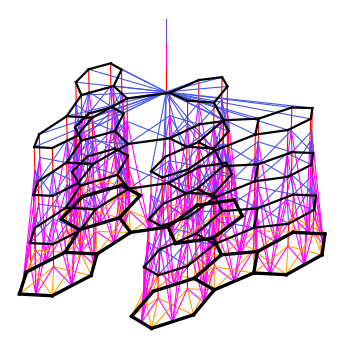
\includegraphics[width=0.4\textwidth]{figures/3d-nets/net1}}
\caption{A visual representation of the neural fingerprint architecture.}
\label{fig:architecture sketch}
\end{figure}

Neural fingerprints offer several advantages over fixed, classical fingerprints:
\begin{itemize}
\item Molecular features can be automatically tuned to the task at hand.
Currently, many hand-engineered variants of circular fingerprints exist for various settings. [cite, and give examples]
\item Better predictive performace[?]
\item Because fixed fingerprints are not adapted to the task at hand, their output vector must be extremely large to encode all possible substructures without overlap.
For example, \cite{unterthinerdeep} used a fingerprint vector of size 43,000 for each molecule, after having removed rarely-occurring features in order to make the problem computationally feasible.
We [hopefully] show that better performance can be achieved using feature vectors a fraction of the size, reducing memory requirements and computational burden.
\item Finally, the architecture presented here opens the door for more sophisticated information-aggregation architectures, such as recursive neural networks [cite].
\end{itemize}


\section{Connection to circular fingerprints}

%Circular fingerprints are designed to capture information about which substructures are present in a molecule in a way that is invariant to atom-relabeling.

Standard circular fingerprints already implement a similar architecture, but the analogy to convolutional neural networks is not obvious.
Circular fingerprints generate each layer's features by applying a fixed hash function to the concatenated features in each neighborhood.
The result of these hashes are then treated as integer indices, where a 1 is written to the feature vector at the index given by the feature vector at each node in the graph.
If there are no collisions in the hash function, then each index represents a particular molecular substructure.
Because the size of the substructures represented by each index depend on the depth of the network, the number of layers is referred to as the `radius' of the fingerprints.

The space of possible network architectures is large, but in the spirit of starting from a known-good configuration, we chose an architecture closely analogous to existing fingerprints.
Our neural fingerprints could reasonably be said to generalize existing fingerprints.
In Section \ref{sec:random is equivalent}, we show that randomly-initialized neural fingerprints have similar performance to existing fingerprints.

\section{Creating a differentiable fingerprint}
This section describes our replacement of each discrete operation in circular fingerprints with a differentiable analogue.

\paragraph{Hashing}
The most straightforward choice in our design is that of replacing the hashing function applied at each neighborhood with a single layer of a neural network.
This raises several design decisions, such as the choice of activation function, and the dimension of the feature vectors.
We make these choices in the standard way, using Bayesian optimization [cite] to optimize cross-validation accuracy.

\paragraph{Indexing}
One striking design aspect of circular fingerprints is the transformation of a feature vector into an index.
In convolutional neural networks, pooling is usually performed on each feature separately.
[more connecting text]
We use the softmax operation as a differentiable analogue of indexing.
We do this for three reasons: 1. To match Morgan fingerprints 2. To ensure sparsity of the fingprint 3. So that each fingerprint has a specific meaning - arbitrary rotations of the weight matrices will not give rise to equivalent models.

\paragraph{Canonicalization}
Circular fingerprints produce the same fingerprints regardless of the ordering of atoms in each neighborhood, by sorting the neighboring atoms according to their features (and bond features).
We experimented with this sorting scheme, and also with applying the local feature transform on all possible permutation of the local neighborhood.
In the interests of simplicity and scalability, we decided to simply sum the local atom and bond features.

Algorithms \ref{alg:ecfp} and \ref{alg:neural} summarize these two algorithms and highlight their differences.

\begin{figure*}[t]
 \begin{minipage}[t]{0.49\columnwidth}
 \begin{algorithm}[H]
\caption{Circular fingerprints} 
\label{alg:ecfp} 
\begin{algorithmic}[1]
\State \textbf{Input:} {molecule, radius $R$, size $S$}
\State \textbf{Initialize:} {fingerprint vector $\vf \leftarrow \vzero_S$}
\For {each atom $a$ in molecule} 
    \State $\vr_a \leftarrow g(a)$ \Comment {lookup atom features}
\EndFor
\For {$L = 1$ to $R$} \Comment {for each layer}
	\For {each atom $a$ in molecule}
		\State $\vr_{n1} \dots \vr_{nN} = \textnormal{neighbors}(a)$
		\State $\vv \leftarrow [\vr_a \vr_{n1} \dots, \vr_{nN}]$ \Comment {concatenate}
		\State $\vr_a \leftarrow \textnormal{hash}(\vv)$ \Comment {hash function}
		\State $i \leftarrow \textnormal{mod}(r_a, S)$ \Comment {convert to index}		
		\State $\vf_{i} \leftarrow 1$ \Comment {Write 1 at index}
	\EndFor
\EndFor
\State \textbf{Return:} {binary vector $\vf$}
\end{algorithmic}
\end{algorithm}
\end{minipage}
\hfill
\begin{minipage}[t]{0.49\columnwidth}
\begin{algorithm}[H]
\caption{Neural fingerprints} 
\label{alg:neural} 
\begin{algorithmic}[1]
\State \textbf{Input:} {molecule, radius $R$, size $S$, {\color{blue} $\theta_1 \dots \theta_R$}}
\State \textbf{Initialize:} {fingerprint vector $\vf \leftarrow \vzero_S$}
\For {each atom $a$ in molecule} 
	\State $\vr_a \leftarrow g(a)$ \Comment {lookup atom features}
\EndFor
\For {$L = 1$ to $R$} \Comment {for each layer}
    \For {each atom $a$ in molecule}
		\State $\vr_{n1} \dots \vr_{nN} = \textnormal{neighbors}(a)$
		\State $\vv \leftarrow [\vr_a \vr_{n1}, \dots \vr_{nN}]$ \Comment {concatenate}
		\State $\vr_a \leftarrow {\color{blue} \vf_{\theta_L}}(v)$ \Comment {{\color{blue} smooth function}}
		\State $\vi \leftarrow \textnormal{{\color{blue}softmax}}(\vr_a)$ \Comment {{\color{blue} sparsify}}
		\State $\vf \leftarrow {\color{blue} \vf + \vi}$ \Comment {{\color{blue}add to fingerprint}}
    \EndFor
\EndFor
\State \textbf{Return:} { {\color{blue} real-valued} vector $\vf$}
\end{algorithmic}
\end{algorithm}
\end{minipage}
\hfill
\caption{Pseudocode of circular fingerprints (\emph{left}) and neural fingerprints (\emph{right}).
Differences are highlighted in blue.
Every non-differentiable operation has been replaced with a differentiable analogue.}
\end{figure*}




\section{Related work}

\paragraph{Neural fingerprints}
The most closely related work is \citet{lusci2013deep}, who also replace circular fingerprints with a neural network having graph-valued inputs.
Their approach is to remove all cycles and build the graph into a tree structure, choosing one atom to be the root.
A recursive neural network~\citep{socher2011dynamic, socher2011semi} is then run from the leaves to the root to produce a fixed-size representation.
The final descriptor is a sum of the representations of all distinct graphs.
There are as many distinct graphs as there are atoms in the network.
The computational cost of this method thus grows as $\mathcal{O}(F^2N^2)$, where $F$ is the size of the feature vector and $N$ is the number of atoms.


\paragraph{Convolutional Neural Networks}

Convolutional neural networks have been used to model images, speech, and time series~\cite{lecun1995convolutional}.
However, standard convolutional architectures use a fixed computational graph, making them difficult to apply to objects of varying size or structure, such as molecules.
More recently, \cite{KalchbrennerACL2014} and others have developed a convolutional neural network architecture for modeling sentences of varying length.


\paragraph{Neural nets for QSAR}

\cite{ramsundar2015massively} Massively multitask networks for drug discovery

\cite{dahl2014multi, ma_qsar_2015} used standard deep neural networks, and didn't do any feature engineering.

\paragraph{Machine learning for identifying promising molecules}

\cite{Eckert2007225, bergeron2011modeling} provide reviews of the field.
\cite{tingley2014towards} used a variety of standard machine learning algorithms to predict the photovoltaic efficiency of organic molecules.

\paragraph{Neural Networks on Graphs}

\cite{graphnn2009} The Graph Neural Network Model

\cite{micheli2009neural} Neural network for graphs

\paragraph{Unrolled inference algorithms}
\citet{hershey2014deep} and [cite CD as unrolled inference] have noted that iterative inference procedures in many models resemble the feedforward computation of a recurrent neural network, or other deep neural networks.
One natural combination of these ideas is to parameterize these inference steps, and train a neural network to approximately match the output of exact inference in a smaller number of iterations.
The neural fingerprint, when viewed in this light, resembles an unrolled message-passing algorithm on the original graph.


\section{Experiments}

We generated molecular graphs from SMILES [cite] using RDkit [cite].
We used the ECFP implementation provided by RDkit.
We used Whetlab [cite].

In our convolutional networks, the initial atom and bond features were chosen to be similar to those used by ECFP.
The atom features were a concatenation of a one-hot encoding of the element, the degree, the number of attached hydrogen atoms, and the implicit valence, and one feature indicating if the atom is in an aromatic ring. 
The bond features were a concatenation of whether the bond type was single, double, triple, or aromatic, whether the bond was conjugated, and whether the bond is part of a ring.

We initially experimented with batch normalization [cite] vs not (on the validation set error!), and since it was almost always superior in practice, we left it on.
We also experimented with tanh vs relu (on the validation set error!), but relu had a slight performance advantage.
We also experimented with dropout, but since it was unhelpful in practice (on the validation set error!) we disabled it. 

\subsection{Randomly initialized neural fingerprints are similar to circular fingerprints}
\label{sec:random is equivalent}

We can answer this question by evaluating the performance of neural fingerprints generated by randomly initialized weights.

\begin{figure}[h]
\centerline{\includegraphics[width=0.5\textwidth]{../../DeepMoleculesData/experiments/2015-05-25-delaney/4-depth-large-small/figures/all_rmses.pdf}}
\caption{A visual representation of the neural fingerprint architecture.}
\label{fig:architecture sketch}
\end{figure}

\subsection{Datasets}

Tripod dataset: \url{https://tripod.nih.gov/tox21/challenge/}
\cite{unterthiner2015toxicity}

Delaney dataset:
\cite{delaney_data_2004}


\subsection{Examining learned features}

Figure \ref{fig:learned features} shows which fragments maximally activated various features.

\newcommand{\molfeature}[2]{\includegraphics[width=3.5cm]{../../DeepMoleculesData/experiments/2015-05-30-visualize-fps/1/figures/fp_#1_highlight_#2.pdf}}%

\begin{figure}[h]
\begin{tabular}{cccc}
Fingerprint 1 & \molfeature{0}{1} & \molfeature{0}{2} & \molfeature{0}{9} \\
Fingerprint 2 & \molfeature{1}{1} & \molfeature{1}{2} & \molfeature{1}{9} \\
Fingerprint 3 & \molfeature{2}{1} & \molfeature{2}{2} & \molfeature{2}{9} \\
Fingerprint 4 & \molfeature{3}{1} & \molfeature{3}{2} & \molfeature{3}{9}
\end{tabular}
\caption{The molecular fragments which most activate the four features of the convolutional net.}
\label{fig:learned features}
\end{figure}

\subsection{Implementation Details}
Automatic differentiation (AD) software packages such as
Theano~\citep{Bastien-Theano-2012, bergstra2010scipy} significantly speed up development time by providing gradients automatically, but can only handle limited control structures and indexing.
Since we required relatively complex control flow and indexing in order to implement variants of Algorithm \ref{alg:neural}, we implemented our own automatic differentiation package for Python, available at \url{<redacted>}.
This package differentiates standard Numpy~\citep{oliphant2007python} code, and can differentiate code containing
while loops, branches, indexing, and even its own gradient evaluations.

Code for all experiments in this paper will be made available upon publication.



\section{Extensions}

\paragraph{How much computation to perform at each layer?}
i.e. how complicated should we make the function that goes from one layer of the graph to the next?

\paragraph{Building parse trees}
For the pyramidal architecture, we need to decide on a parse tree of the molecule.
One way to do this in a 'soft' way might be to max-pool over many different local parsings.
This could be done at multiple layers, which would limit the exponential blowup.

\paragraph{Preserve asymmetries explicitly or implicitly}
If we tie the weights of all neighboring vertices, then ordering information is lost locally, although it is still preserved implicitly in the relations between nodes in the next layer.

\paragraph{3D features}
How to extend this to using 3d features?

\subsection{Interpretability}
[Idea: Use nested dropout to allow a variable-sized descriptor.]
Explain that it's analogous to PCA for neural nets

[Wishlist: Include figures showing which fragments maximally activate different features - hopefully showing that they correspond to interpretable, familiar concepts]

\paragraph{Using LSTMs instead of RNNs}


\section{Conclusions}


%\section*{Acknowledgments}



\bibliography{references.bib}
\bibliographystyle{include/icml2015}



\end{document}